\section{快速冪}
    \subsection{前言}
    看到快速冪,你應該會先想到:「什麼是冪。」

    答案是次方,就是形如$a^x$的東西。一般而言,我們可能會想說計算$a^x$需要$O(x)$的時間,因為需要$n-1$次乘法。程式如下。

\begin{lstlisting}[caption=慢速冪]
int POW(int a,int x){
    int ret=1;
    for(int i=0;i<x;++i){
        ret*=a;
    }
    return ret;
}
\end{lstlisting}

    \subsection{概念}
    我們其實可以透過一些方法減少需要的方法數,特別是如果我們的$x$滿足$x=2^k, k \in \N$時。因為我們可以用$a \times a$獲得$a^2$,
    再使用$a^2 \times a^2$得到$a^4$,依此類推,我們只需要使用$O(\log{x})$的時間就可以完成。

    但如果計算$a^n$的時候$n \notin \N$呢?不用慌,我們同樣可以用一些的方法算出答案。而且不超過$O(\log{(n)})$。
    我們可以將$n$轉換成二進位,例如$10_{(10)}$就可以表示為$1010_{(2)}$。如果要計算$a^{10}$。利用剛剛的方法就可以得到$a^2$以及$a^8$。
    最後將兩者相乘,$a^{10}$ get!。

    \subsection{實作}
    實作上我們可以使用while或者遞迴,因為迴圈常數比較小,所以我比較常用。不過實際上應該不會因為這樣被卡常數,所以也還好。

\begin{lstlisting}[caption=迴圈快速冪]
int POW(int a,int x){
    int ret=1;
    while(x>0){
        if(x&1){// => if(x%2==1)
            ret*=a;
        }
        a*=a;
        x>>=1;// => x/=2;
    }
}
\end{lstlisting}

    這份程式碼反覆利用\verb|x%2==1|以及\verb|x/=2|完成對$x_{(2)}$的從右邊數過來第$k$位數是否為$1$的偵測。

    \subsection{應用}
    通常來說,快速冪計算的數字都非常大,大到long long也裝不下,那究竟有什麼樣的用途呢?
    其實,程式競賽大多會請你對一個數字取餘,一般是$10^{9}+7$。我習慣用常數而非巨集。

\begin{lstlisting}
using ll=long long;
const ll MOD=1e9+7;
\end{lstlisting}

    \subsection{範例與練習}
    \problem 請使用請使用遞迴方法實作快速冪。

    \problem 請實作對於$(a+b\sqrt{2})^{n}$的快速冪算法。

    \problem 請實作對於$(a\sqrt{2}+b\sqrt{6})^{n}$的快速冪算法。

    \example 設計時間複雜度為$O(n\log{(n)})$的費氏數列算法。

    關於這個問題,首先我們可以思考,如果要計算$a_n$,我們就需要$a_{n-1}$和$a_{n-2}$。
    於是我們可以用矩陣來表示相鄰項之間的關係式。

    $$\begin{bmatrix}
        a_n \\
        a_{n-1}
    \end{bmatrix}
    =
    \begin{bmatrix}
        1 & 1 \\
        1 & 0
    \end{bmatrix}
    \times 
    \begin{bmatrix}
        a_{n-1} \\
        a_{n-2}
    \end{bmatrix}$$

    此矩陣乘法表示兩件事。首先是$a_n=1 \times a_{n-1}+1 \times a_{n-2}$,另一個是$a_{n-1}=1 \times a_{n-1}+0 \times a_{n-2}$。

    這樣表示有什麼好處呢?沒錯,既然

    $$\begin{bmatrix}
        a_n \\
        a_{n-1}
    \end{bmatrix}
    =
    \begin{bmatrix}
        1 & 1 \\
        1 & 0
    \end{bmatrix}
    \times 
    \begin{bmatrix}
        a_{n-1} \\
        a_{n-2}
    \end{bmatrix}$$

    那麼 

    $$\begin{bmatrix}
        a_n \\
        a_{n-1}
    \end{bmatrix}
    =
    \begin{bmatrix}
        1 & 1 \\
        1 & 0
    \end{bmatrix}^{2}
    \times 
    \begin{bmatrix}
        a_{n-2} \\
        a_{n-3}
    \end{bmatrix}$$

    直接重複$n-2$次,我們就會得到。

    $$\begin{bmatrix}
        a_n \\
        a_{n-1}
    \end{bmatrix}
    =
    \begin{bmatrix}
        1 & 1 \\
        1 & 0
    \end{bmatrix}^{n-2}
    \times 
    \begin{bmatrix}
        a_2 \\
        a_1
    \end{bmatrix}
    =
    \begin{bmatrix}
        1 & 1 \\
        1 & 0
    \end{bmatrix}^{n-2}
    \times 
    \begin{bmatrix}
        1 \\
        1
    \end{bmatrix}
    $$

    實作前,我們先處理矩陣乘法的問題,這可以透過下面方式解決。

\begin{lstlisting}[caption=矩陣乘法$O(n^3)$]
using ll=long long;
using vec=vector<ll>;
using Mer=vector<vec>;
const ll MOD=1e9+7;

Mer operator*(Mer a,Mer b){
    Mer ret(a.size(),vll(b[0].size()));
    for(int i=0;i<a.size();++i){
        for(int j=0;j<b[0].size();++j){
            for(int k=0;k<a.size();++k){
                ret[i][j]=(ret[i][j]+a[i][k]*b[k][j])%MOD;
            }
        }
    }
    return ret;
}
\end{lstlisting}

    使用迴圈實作時,應該要注意單位矩陣的形式。否則將產生錯誤。

\begin{lstlisting}[caption=矩陣快速冪]
Mer POW(Mer a,ll x){
    Mer ret(a.size(),vll(a[0].size(),0));
    for(int i=0;i<a.size();++i) ret[i][i]=1;
    while(x>0){
        if(x&1) ret=ret*a;
        a=a*a;
        x>>=1;
    }
    return ret;
}
\end{lstlisting}

    有了這樣的工具之後,計算費氏數列就變得很容易。我們可以輕易的使用POW解決這個問題。

\begin{lstlisting}[caption=費氏數列$O(\log{(n)})$算法]
int calculate(ll n){
    Mer t={
        {1,1},
        {1,0}
    };

    t=POW(t,n-2);

    Mer ori={
        {1},
        {1}
    };

    Mer ans=t*ori;

    return ans[0][0];
}    
\end{lstlisting}

    \problem 有一個數列$a$滿足以下遞迴式,試表示其矩陣轉移式。

    $$
    \begin{cases}
        a_1=1, \; a_2=2 \\
        a_n=x \times a_{n-1} + y \times a_{n-2}, \; n \ge 2
    \end{cases}
    $$

    \problem 第一屆卓越盃 E.Steal A Safe

    \textbf{題目敘述}

    宜中偷分大師現在想偷點不同的東西了,為了證明自己的實力,他決定偷裡面僅有一個寫著卓岳的馬克杯的保險箱,這個保險箱是一個正方體,大致如圖。

    \begin{figure}[h]
        \centering
        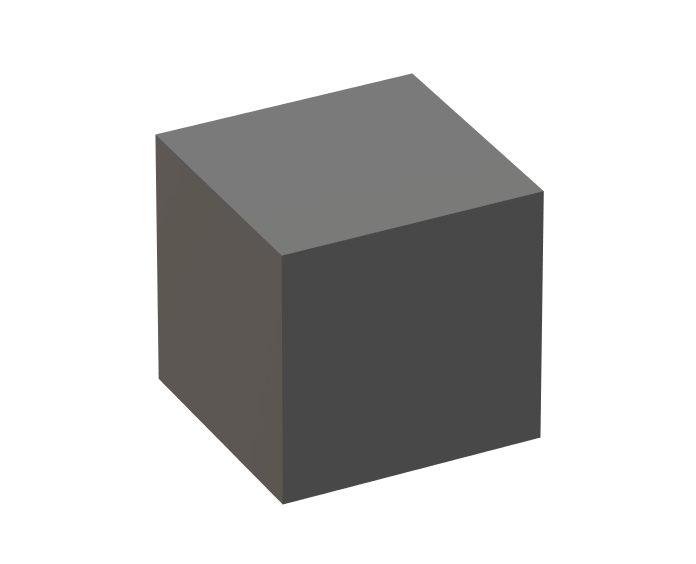
\includegraphics[width=0.7\textwidth]{../Images/StealASafe.png}
    \end{figure}

    上面有一個密碼鎖(請原諒我畫不出來),卻沒有重置密碼的按鈕,因此他認為此保險箱的密碼是固定的。這時,他發現保險箱側邊有一個類似金字塔的東西,用的是不同的金屬。用電子顯微鏡一看,竟發現上面有規律地排列。然而以他薄弱的計算能力,他認為他一定會算錯。而且金字塔的層數過多,增長又很快,更是讓他打消手算的念頭。然而他不會寫程式,因而請你幫忙。

    為了避免讓你花太多時間(後面還有題目),他已經幫你把他們的遞迴關係式列出來了,如下。

    $$
    \begin{cases}
    S_1=x_1, \, S_2=x_2\\
    S_n=a \times S_{n-1} + b \times S_{n-2} + cn^2 + d \times 2^n\\
    \end{cases}
    $$

    很明顯這個數字會很大,因此他猜想可能要對某數取餘。且因保險箱的設計者是一個常年在 $ICPC$ 破台的高手,因此他猜模數 $(M)$ 應該是 $10^9+7$ 或是 $998244353$ 。請算出 $n$ 層的原子數(記得對 $M$ 取餘)。

    \textbf{輸入說明}

    第一行輸入 $t$。
    接著輸入 $t$ 行,每行 $8$ 個數字,分別為 $x_1 \; x_2 \; a \; b \; c \; d \; n \; M$ ,其意義如上所述。

    $t \le 10^3$

    $x_1, \; x_2 \le 10^3$

    $a, \; b, \; c, \; d \le 100$

    $n \le 10^{12}$
    
    $M \in \{\, 10^9+7,998244353 \,\}$

    \textbf{輸出說明}

    輸出 $t$ 個數字 $S_n$ (記得對 $M$ 取餘),數字間要換行。

    \textbf{範例測試}

    \begin{tabular}{|m{9.5cm}|m{4.5cm}|}
        \hline
        範例輸入 1 & 範例輸出 1 \\
        \hline
        \verb|1| &  \verb|2| \\
        \verb|1 1 1 1 0 0 3 1000000007| & \\
        \hline
        範例輸入 2 & 範例輸出 2 \\
        \hline
        \verb|2| &  \verb|857215810| \\
        \verb|727 434 77 62 32 82 977211338887 1000000007| & \verb|31| \\
        \verb|1 1 2 3 2 1 3 1000000007| & \\
        \hline
    \end{tabular}